\documentclass[11pt,openany]{article}

\input{algebra-preamble}
\usepackage{commath}
\usepackage{caption}
%Tikzpicture
\usepackage{tikz}
\usepackage{tikz-3dplot}
\usepackage{tikz-cd}
\usetikzlibrary{
	3d, % For 3D drawing
	angles,
	arrows,
	arrows.meta,
	backgrounds,
	bending,
	calc,
	decorations.pathmorphing,
	decorations.pathreplacing,
	decorations.markings,
	fit,
	matrix,
	patterns,
	patterns.meta,
	positioning,
	quotes,
	shadows,
	shapes,
	shapes.geometric
}
\input{../preamble/tcolorbox}

\newcommand{\arrowboth}[1][]{\arrow[#1, bend left=15, myarrow]\arrow[bend left=15, myarrow, from=#1]}
\newcommand{\topology}{\mathcal{T}}

\usepackage{multirow}
\usepackage{xcolor,cancel}

\newcommand\hcancel[2][black]{\setbox0=\hbox{$#2$}%
	\rlap{\raisebox{.45\ht0}{\textcolor{#1}{\rule{\wd0}{1pt}}}}#2} 

\setstretch{1.25}
\begin{document}
	\pagenumbering{arabic}
	\begin{center}
		\huge\textbf{Topology for Polynomial Rings}\\
		\vspace{0.5em}
		%	\Large\quad{대수학의 아름다움 서브-스터디}\\
		\vspace{0.5em}
		\normalsize{\today}\\
	\end{center}
	\begin{itemize}
		\item $\C$: Field of Complex Numbers
		\item $\mathbb{K}$: Field
		\item $\textbf{x}:=(x_1,\dots,x_n)$
		\item $X:=\mathbb{K}^n$
	\end{itemize}
	\adjustbox{scale=.9}{\setstretch{1.75}
		\begin{tabular}{|l||c|c|c|} \hline
			\textbf{Polynomial Ring (Set)} & $\C[x]$ & $\C[x,y]$ & $\mathbb{K}[x_1,\dots,x_n]$ \\ \hline\hline
			\multirow{2}{*}{\textbf{Element}} & $f\in\C[x]$ & $g\in\C[x,y]$ & $p\in\mathbb{K}[x_1,\dots,x_n]$\\ \cline{2-4}
			& $\fullfunction{f}{\C}{\C}{z}{f(z)}$ & $\fullfunction{g}{\C^2}{\C}{(\alpha,\beta)}{g(\alpha,\beta)}$ & $\fullfunction{p}{X}{\mathbb{K}}{\textbf{x}}{p(\textbf{x})}$\\ \hline\hline
			\textbf{Zero Set} & $Z(f)=\set{z\in\C:f(z)=0}$ & $Z(g)=\set{(\alpha,\beta)\in\C^2:f(\alpha,\beta)=0}$ & $Z(p)=\set{\textbf{x}\in X:p(\textbf{x})=0}$ \\ \hline
	\end{tabular}}
	\begin{center}
	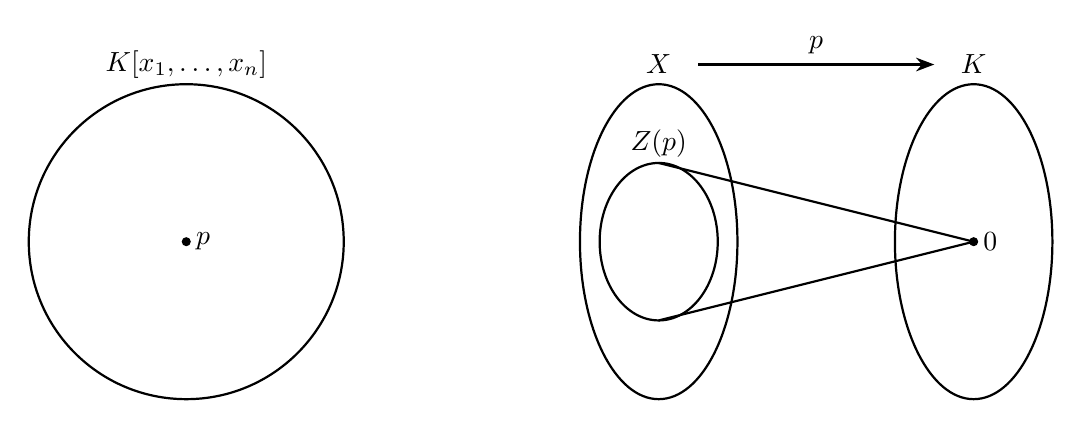
\begin{tikzpicture}
		% Draw the sets A and B
		\draw[thick] (-8,0) ellipse (2 and 2);
		\draw[thick] (-2,0) ellipse (1 and 2);
		\draw[thick] (-2,0) ellipse (.75 and 1);
		\draw[thick] (2,0) ellipse (1 and 2);
		
		% Labels for sets
		\node at (-8, 2.25) {$\mathbb{K}[x_1,\dots,x_n]$};
		\node at (-2, 2.25) {$X$};
		\node at (-2, 1.25) {$Z(p)$};
		\node at (2, 2.25) {$\mathbb{K}$};
		
		% Draw the arrows representing the function
		\draw[-Stealth, thick] (-1.5, 2.25) -- (1.5,2.25) node[midway, above] {$p$};
		
		\draw[fill] (-8,0) circle (.05) node[right] {$p$};
		\draw[fill] (2,0) circle (.05) node[right] {0};
		
		\draw[-, thick] (-2, 1) -- (2, 0);
		\draw[-, thick] (-2, -1) -- (2, 0);
	\end{tikzpicture}
	\end{center}
	For any set of polynomials $S\subseteq\mathbb{K}[x_1,\dots,x_n]$, the \textbf{zero set} $Z(S)$ is defined as: \[
	\boxed{Z(S):=\set{\textbf{x}\in X:p(\textbf{x})=0\ \text{for all}\ p\in S}}.
	\]
	\begin{center}
	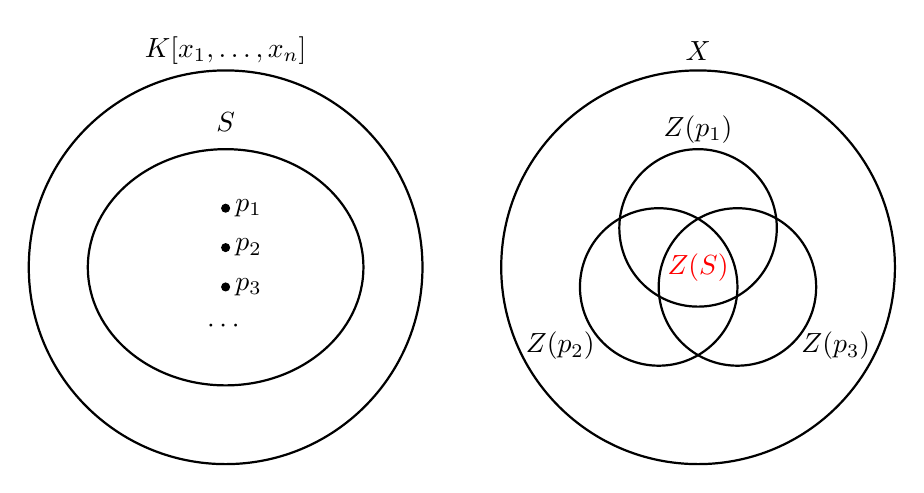
\begin{tikzpicture}
		% Draw the sets A and B
		
		\draw[thick] (-8,0) ellipse (2.5 and 2.5);
		\draw[thick] (-8,0) ellipse (1.75 and 1.5);
		\draw[thick] (-2,0) ellipse (2.5 and 2.5);
		
		\draw[thick] (-2,.5) ellipse (1 and 1);
		\draw[thick] (-1.5,-.25) ellipse (1 and 1);
		\draw[thick] (-2.5,-.25) ellipse (1 and 1);
		
		% Labels for sets
		\node at (-8, 2.75) {$\mathbb{K}[x_1,\dots,x_n]$};
		\node at (-8, 1.85) {$S$};
		\node at (-2, 2.75) {$X$};
		\node at (-2, 1.75) {$Z(p_1)$};
		\node at (-3.75, -1) {$Z(p_2)$};
		\node at (-.25, -1) {$Z(p_3)$};
		\node at (-2, 0) {$\textcolor{red}{Z(S)}$};
		
		% Draw the arrows representing the function
%		\draw[-Stealth, thick] (-1.5, 2.25) -- (1.5,2.25) node[midway, above] {$p$};
		
		\draw[fill] (-8,.75) circle (.05) node[right] {$p_1$};
		\draw[fill] (-8,.25) circle (.05) node[right] {$p_2$};
		\draw[fill] (-8,-.25) circle (.05) node[right] {$p_3$};
		\draw[fill] (-8,-.75) node[] {$\cdots$};
	\end{tikzpicture}
	\end{center}
	Consider \[
	\hcancel[red]{\mathcal{T}:=\set{Z(p)\subseteq X:p\in\mathbb{K}[x_1,\dots,x_n]}\subseteq 2^X}
	\]\[
	\mathcal{T}:=\set{Z(S)\subseteq X:S\subseteq\mathbb{K}[x_1,\dots,x_n]}\subseteq 2^X
	\] We claim that $\mathcal{T}$ is a topology on $X$:
	\begin{itemize}
		\item[(i)] \textbf{(Whole Space and Empty Set)}
		\begin{itemize}
			\item \textcolor{blue}{Let $S=\emptyset$}. By the definition, \[
			Z(\emptyset)=\set{\textbf{x}\in X:p(\textbf{x})=0\ \text{for all}\ p\in\emptyset}.
			\] Therefore, $Z(\emptyset)=X\in\mathcal{T}$ since the condition is vacuously true for every point $\textbf{x}\in X$.
			\item \textcolor{blue}{Let $S=\set{1}$}, where $1\in\mathbb{K}[x_1,\dots,x_n]$. Then \[
			Z(\set{1})=\set{\textbf{x}\in X:1=0}=\emptyset\in\mathcal{T}.
			\]
		\end{itemize}
		\vspace{4pt}
		\item[(ii)] \textbf{(Arbitrary Intersections)} Consider $\set{Z(S_i)}_{i\in\Lambda}\subseteq\mathcal{T}$, where each $Z(S_i)$ is the zero set of some set of polynomials $S_i\subseteq\mathbb{K}[x_1,\dots,x_n]$. Then \begin{align*}
			\bigcap_{i\in\Lambda} Z(S_i)&=\set{\textbf{x}\in X:\textbf{x}\in Z(S_i)\ \text{for all}\ i\in\Lambda}\\
			&=\set{\textbf{x}\in X:p(\textbf{x})=0\ \text{for all}\ p\in S_i\ \text{and for all}\ i\in\Lambda}\\
			&=\set{\textbf{x}\in X:p(\textbf{x})=0\ \text{for all}\ p\in\bigcup_{i\in\Lambda}S_i} \\
			&=Z\of{\bigcup_{i\in\lambda}S_i}
		\end{align*}
		\textcolor{blue}{Let $S:=\bigcup_{i\in\Lambda}S_i\subseteq\mathbb{K}[x_1,\dots,x_n]$}. Then \begin{align*}
			\bigcap_{i\in\Lambda}Z(S_i)=Z\of{\bigcup_{i\in\Lambda}S_i}=Z(S)\in\mathcal{T}.
		\end{align*}
		\vspace{4pt}
		\newpage
		\item[(iii)] \textbf{(Finite Unions)} Consider two zero sets $Z(S_1)$ and $Z(S_2)$, where $S_1,S_2\subseteq\mathbb{K}[x_1,\dots,x_n]$. Then
		\begin{align*}
			Z(S_1)\cup Z(S_2)&=\set{\textbf{x}\in X:\textbf{x}\in Z(S_1)\ \text{or}\ \textbf{x}\in Z(S_2)} \\
			&=\set{\textbf{x}\in X:p(\textbf{x})=0\ \text{for all}\ p\in S_1\ \text{or}\ q(\textbf{x})=0\ \text{for all}\ q\in S_2} \\
			&=\set{\textbf{x}\in X:(p\cdot q)(\textbf{x})=0\ \text{for all}\ p\in S_1\ \text{and for all}\ q\in S_2}
		\end{align*}
		\textcolor{blue}{Let} \[
		\textcolor{blue}{S:=\set{p\cdot q\in\mathbb{K}[x_1,\dots,x_n]:p\in S_1\ \text{and}\ q\in S_2}\subseteq\mathbb{K}[x_1,\dots,x_n]}.
		\] Then \begin{align*}
			Z(S_1)\cup Z(S_2)&=\set{\textbf{x}\in X:(p\cdot q)(\textbf{x})=0\ \text{for all}\ p\in S_1\ \text{and for all}\ q\in S_2}\\
			&=\set{\textbf{x}\in X:(p\cdot q)(\textbf{x})=0\ \text{for all}\ p\cdot q\in S} \\
			&=Z(S)\in\mathcal{T}.
		\end{align*}
	\end{itemize} Hence it is proved
	\begin{flushright}
		$\qed$
	\end{flushright}
\end{document}
